% https://panthema.net/2013/0627-TikZ-Pythagoras-Tree/
% Draw Pythagoras Trees using TikZ
% Author: Timo Bingmann <tb@panthema.net>, 2013-06-27
\documentclass[a4paper]{article}

\usepackage{tikz}

% recursively draw a Pythagoras Tree fractal
% \PythagorasTree{levels}{angle}
\newcommand{\PythagorasTree}[2]{%
  \ifnum#1=0\else
    % randomly pick a color, prefer green and blue shades
    \pgfmathsetmacro{\r}{0.6*rnd}
    \pgfmathsetmacro{\g}{0.9*rnd}
    \pgfmathsetmacro{\b}{0.7*rnd}
    \definecolor{MyColor}{rgb}{\r,\g,\b}

    % draw the rectangle of this level
    \draw[draw=MyColor] (0,0) rectangle (1,1);

    % decrement level counter
    \pgfmathtruncatemacro{\next}{#1-1}

    % transform scope for left branch: move origin (1cm,0cm), rotate and scale
    % with the length of the left cathetus.
    \begin{scope}[
      yshift=1cm,xshift=0cm,
      rotate=#2,scale={cos(#2)}
      ]
      \PythagorasTree{\next}{#2}
    \end{scope}

    % now for the tricks: transform scope for right branch: move origin to the
    % top point of the triangle, rotate reverse and scale with length of right
    % cathetus.
    \begin{scope}[
      yshift={1cm * (1 + sin(#2)*cos(#2))},
      xshift={1cm * (cos(#2)*cos(#2))},
      rotate={#2-90},scale={sin(#2)}
      ]
      \PythagorasTree{\next}{#2}
    \end{scope}
  \fi
}

\begin{document}

% draw just a single Pythagoras Tree
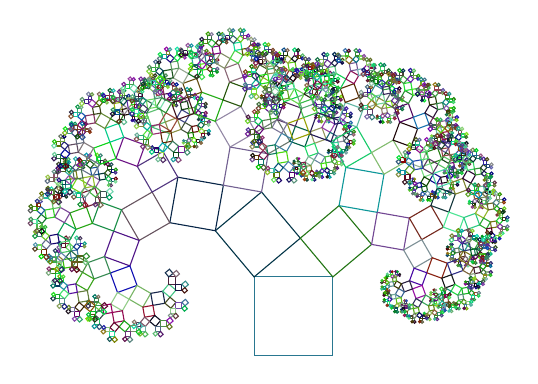
\begin{tikzpicture}[scale=1.0]
  % recursively draw tree
  \PythagorasTree{11}{40}
\end{tikzpicture}\qquad
% draw just a single Pythagoras Tree
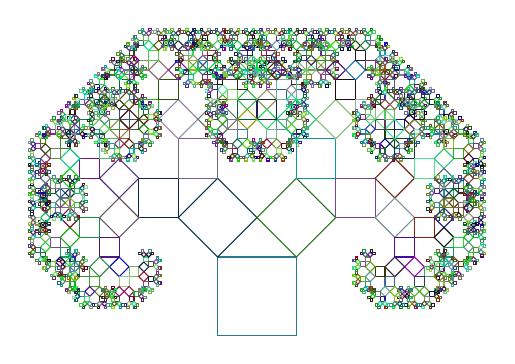
\begin{tikzpicture}[scale=1.0]
  % recursively draw tree
  \PythagorasTree{11}{45}
\end{tikzpicture}

% draw just a single Pythagoras Tree
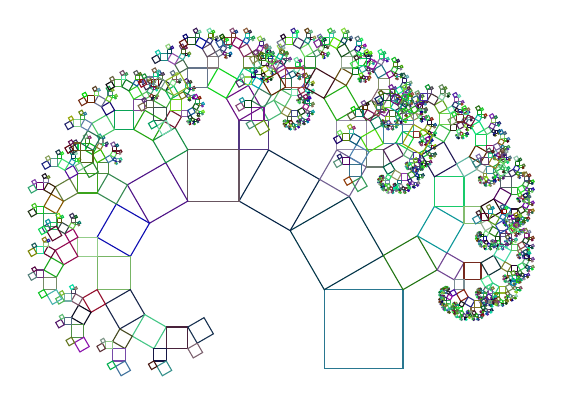
\begin{tikzpicture}[scale=1.0]
  % recursively draw tree
  \PythagorasTree{11}{30}
\end{tikzpicture}\qquad
% draw just a single Pythagoras Tree
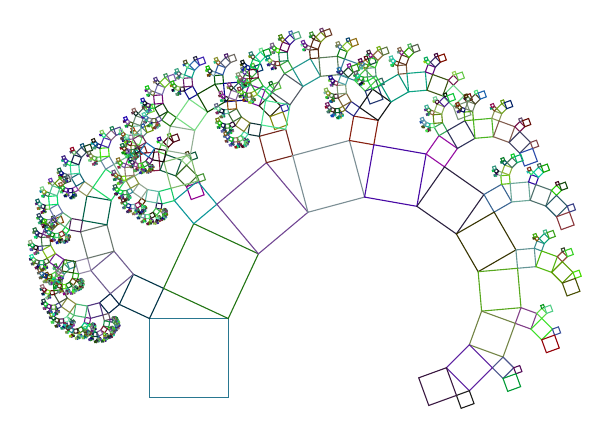
\begin{tikzpicture}[scale=1.0]
  % recursively draw tree
  \PythagorasTree{11}{65}
\end{tikzpicture}

\end{document}

%%% Local Variables:
%%% mode: latex
%%% TeX-master: t
%%% End:
